% This work is licensed under the Creative Commons
% Attribution-NonCommercial 3.0 Unported License. To view a copy of this
% license, visit http://creativecommons.org/licenses/by-nc/3.0/.

\section{Auswertung}
\subsection{Längenmessung}
Es werden die Längen von vier verschiedenen Koaxialkabeln bestimmt.
Dazu wird der zeitliche Abstand zwischen einlaufendem und reflektierten
Signal auf einem Oszilloskop betrachtet.  In den
Abbildungenn~\ref{fig:laenge_rot},~\ref{fig:laenge_schwarz},
~\ref{fig:laenge_gruen} und ~\ref{fig:laenge_trommel} sind die
verwendeten Bilder zu sehen. Die Zeitmessung wird an den dort rot
eingezeichneten Markierungen vorgenommen.  In
Tabelle~\ref{tab:laengenmessung} sind die abgelesenen Zeitabstände
eingetragen. Ebenso in dieser Tabelle sind die mit den Zeitabständen mit
Hilfe von Formel~\eqref{eq:laenge} errechneten Längen der Kabel
eingetragen.  Die Dielektrizitätszahl der Kabel wird mit
$\epsilon_\text{r} = \num{2.25}$ angenommen.\\
Der Fehler der Kabellänge wird mit einer Gausschen 
Fehlerfortpflanzung bestimmt, welche in 
Gleichung~\eqref{eq:gausslaenge} angegeben ist.\\
%
\begin{equation}
\delta L = \frac{c_0}{2\sqrt{\epsilon_\text{r}}}\delta t
\label{eq:gausslaenge}
\end{equation}
%
\begin{table}[h]
  \centering
  \begin{tabular}{SSS}
    \toprule
    {Kabel}&{Signalabstand }$\Delta${t/}\si{\nano\second}&{Kabellänge/}\si{\metre}\\
    \midrule
    {Rot}&18(2)&1.8(2)\\
    {Schwarz}&116(12)&11.6(12)\\
    {Grün}&85(9)&8.5(9)\\
    {Trommel}&822(82)&82.1(82)\\
    \bottomrule
  \end{tabular}
  \caption{Mit dem Oszilloskop wurden die zeitlichen Abstände 
    zwischen einlaufendem und reflektiertem Signal bestimmt.  Die
    Kabellängen sind mit Formel~\eqref{eq:laenge} berechnet worden.}
  \label{tab:laengenmessung}
\end{table}
%
\begin{figure}
  \centering

  \begin{subfigure}{0.4\textwidth}
    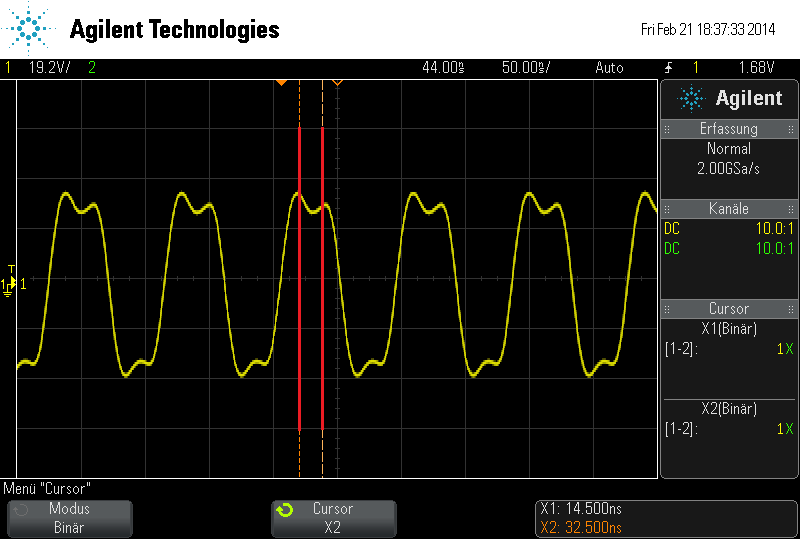
\includegraphics[width=\textwidth]{laenge_rot.png}
    \caption{rotes Kabel}
    \label{fig:laenge_rot}
  \end{subfigure}
  \quad
  \begin{subfigure}{0.4\textwidth}
    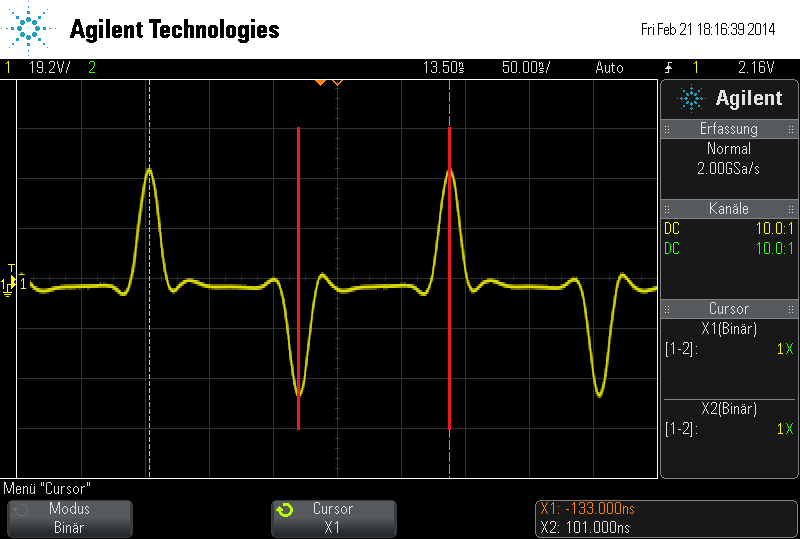
\includegraphics[width=\textwidth]{laenge_schwarz.png}
    \caption{schwarzes Kabel}
    \label{fig:laenge_schwarz}
  \end{subfigure}

  \begin{subfigure}{0.4\textwidth}
    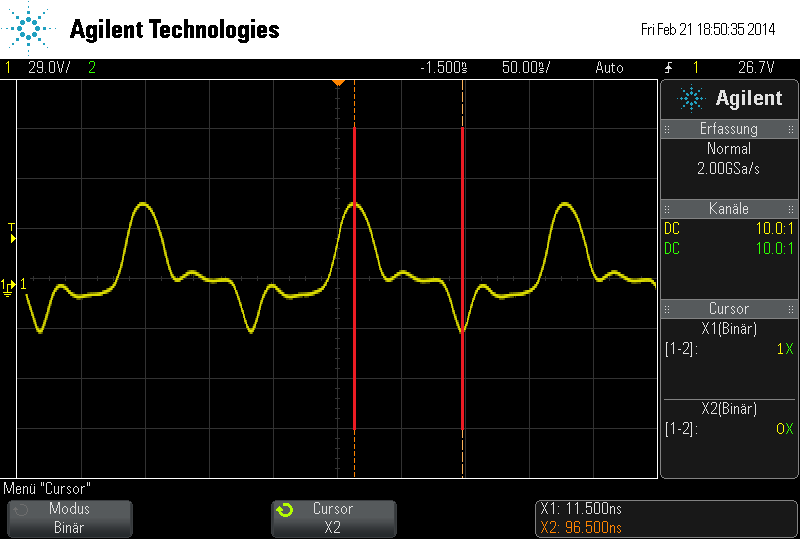
\includegraphics[width=\textwidth]{laenge_gruen.png}
    \caption{grünes Kabel}
    \label{fig:laenge_gruen}
  \end{subfigure}
  \quad
  \begin{subfigure}{0.4\textwidth}
    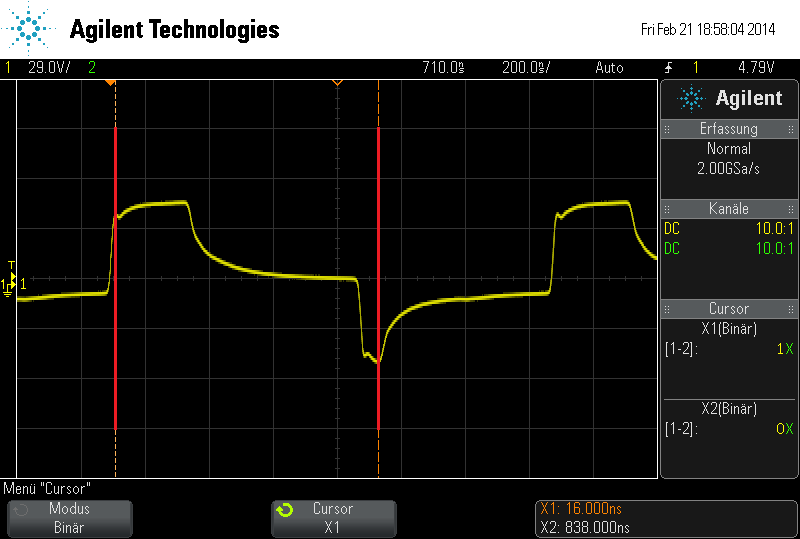
\includegraphics[width=\textwidth]{laenge_trommel.png}
    \caption{Kabeltrommel}
    \label{fig:laenge_trommel}
  \end{subfigure}

  \caption{Aufgenommene Oszilloskopenbilder zur Bestimmung der
    jeweiligen Kabellängen. Der zeitliche Abstand der Signale wird an
    den roten Markierungen abgelesen.}
\end{figure}

\subsection{Belagsmessung}
%
Die mit einem LRC-Messgerät bestimmten Induktivitäten ${L}_\text{g}$,
Widerstände ${R}_\text{g}$ und Kapazitäten ${C}_\text{g}$ bei
verschiedenen Frequenzen $f$ sind für das rote Kabel in
Tabelle~\ref{tab:RLC_rot}, für das schwarze Kabel in
Tabelle~\ref{tab:RLC_schwarz}, und für die Kabeltrommel in
Tabelle~\ref{tab:RLC_trommel} aufgeführt.  Ebenfalls in diesen Tabellen
sind sowohl die mit Formel~\eqref{eq:belagsformel} berechneten
Querleitwerte ${G}_\text{g}$ der jeweiligen Kabel aufgeführt, als auch
die durch die Längen der Kabel errechneten Beläge $R, L, C$ und $G$.
%
\begin{table}[h]
  \centering
  \sisetup {
    per-mode = fraction
  }
  \begin{tabular}{SSSSSSSSS}
    \toprule
    {f /}\si{\kilo\hertz}&
    ${R}_\text{g}${/}\si{\ohm}&{R/}\si{\ohm\per\metre}&
    ${L}_\text{g}${/}\si{\micro\henry}&{L/}\si{\micro\henry\per\metre}&
    ${C}_\text{g}${/}\si{\pico\farad}&{C/}\si{\pico\farad\per\metre}&
    ${G}_\text{g}${/}\si{\micro\siemens}&{G/}\si{\micro\siemens\per\metre}\\
    \midrule
    0.05&2.47&1.37&4.5&2.50&138.8&77.2&76.2&42.4\\
    0.10&2.48&1.38&4.5&2.50&138.8&77.2&76.5&42.5\\
    0.20&2.48&1.38&4.4&2.45&138.8&77.2&78.2&43.5\\
    0.30&2.48&1.38&4.6&2.56&138.8&77.2&74.8&41.6\\
    0.50&2.48&1.38&4.5&2.50&138.8&77.2&76.5&42.5\\
    0.80&2.48&1.38&4.3&2.40&138.8&77.2&80.0&44.5\\
    1.00&2.49&1.38&4.2&2.33&138.8&77.2&82.3&45.7\\
    1.50&2.49&1.38&4.1&2.28&138.8&77.2&84.3&46.9\\
    2.00&2.50&1.39&4.0&2.22&138.7&77.1&86.7&48.2\\
    3.00&2.51&1.40&3.8&2.10&138.7&77.1&92.3&51.3\\
    5.00&2.53&1.41&3.4&1.89&138.6&77.1&103.1&57.3\\
    7.00&2.55&1.42&3.2&1.78&138.6&77.1&110.4&61.4\\
    10.00&2.56&1.42&3.0&1.67&138.6&77.1&118.3&65.8\\
    14.00&2.58&1.43&2.8&1.56&138.5&77.0&127.6&70.9\\
    18.00&2.59&1.44&2.8&1.56&138.5&77.0&128.1&71.2\\
    20.00&2.60&1.45&2.7&1.50&138.5&77.0&133.4&74.1\\
    100.00&2.60&1.45&2.6&1.45&138.6&77.1&138.6&77.1\\
    \midrule
     \multicolumn{2}{c}{Literaturwert}&0.8&\%&\%&\%&63.0&\%&\%\\
    \bottomrule
  \end{tabular}
  \caption{Mit dem RLC-Messgerät gemessene Widerstands-, 
    Induktivitäts- und Kapazitätswerte für verschiedene Frequenzen 
    des Sinussignals des Messgeräts für das rote Kabel. 
    Aus diesen wird der Querleitwiderstand berechnet. 
    Aus der oben bestimmten Länge des 
    Kabels werden schlussendlich die Beläge bestimmt.
    Die Literaturwerte werden aus \cite{kabel-kusch} für ein 
    Rg 179 B/U Kabel entnommen.}
  \label{tab:RLC_rot}
\end{table}
%
\begin{table}[h]
\small
  \centering
  \sisetup {
    per-mode = fraction
  }
  \begin{tabular}{SSSSSSSSS}
    \toprule
    {f /}\si{\kilo\hertz}&
    ${R}_\text{g}${/}\si{\ohm}&{R/}\si{\ohm\per\metre}&
    ${L}_\text{g}${/}\si{\micro\henry}&{L/}\si{\micro\henry\per\metre}&
    ${C}_\text{g}${/}\si{\pico\farad}&{C/}\si{\pico\farad\per\metre}&
    ${G}_\text{g}${/}\si{\micro\siemens}&{G/}\si{\micro\siemens\per\metre}\\
    \midrule
    0.05&2.41&0.21&8.8&0.76&1100&94.9&301.3&26.0\\
    0.10&2.41&0.21&7.3&0.63&988&85.2&326.2&28.1\\
    0.20&2.41&0.21&7.1&0.61&988&85.2&335.4&29.0\\
    0.30&2.41&0.21&7.0&0.60&988&85.2&340.2&29.3\\
    0.50&2.41&0.21&7.2&0.62&988&85.2&330.7&29.0\\
    0.80&2.41&0.21&7.0&0.60&988&85.2&340.2&29.3\\
    1.00&2.41&0.21&6.9&0.59&988&85.2&345.1&29.8\\
    1.50&2.41&0.21&6.8&0.59&988&85.2&350.2&30.2\\
    2.00&2.41&0.21&6.7&0.58&988&85.2&355.4&30.7\\
    3.00&2.42&0.21&6.4&0.55&988&85.2&373.6&32.2\\
    5.00&2.43&0.21&6.0&0.52&988&85.2&400.1&34.5\\
    7.00&2.44&0.21&5.8&0.50&988&85.2&415.6&35.9\\
    10.00&2.45&0.21&5.6&0.48&988&85.2&432.3&37.3\\
    14.00&2.45&0.21&5.5&0.47&988&85.2&440.1&38.0\\
    18.00&2.46&0.21&5.4&0.47&988&85.2&450.1&38.8\\
    20.00&2.46&0.21&5.4&0.47&988&85.2&450.1&38.8\\
    100.00&2.60&0.22&5.2&0.45&990&85.4&495.0&42.7\\
    \midrule
     \multicolumn{2}{c}{Literaturwert}&0.05&\%&\%&\%&100.0&\%&\%\\
    \bottomrule
  \end{tabular}
  \caption{In dieser Tabelle sind die gleichen Daten 
    wie in Tabelle~\ref{tab:RLC_rot} eingetragen. Hier aber 
    für das schwarze Kabel. Es handelt sich um den Kabeltyp Rg 
    58 C/U. Die Literaturwerte stammen aus \cite{faberkabel}.}
  \label{tab:RLC_schwarz}
\end{table}
%
\begin{table}[h]
\small
  \centering
  \sisetup {
    per-mode = fraction
  }
  \begin{tabular}{SSSSSSSSS}
    \toprule
    {f /}\si{\kilo\hertz}&
    ${R}_\text{g}${/}\si{\ohm}&{R/}\si{\ohm\per\metre}&
    ${L}_\text{g}${/}\si{\micro\henry}&{L/}\si{\micro\henry\per\metre}&
    ${C}_\text{g}${/}\si{\nano\farad}&{C/}\si{\nano\farad\per\metre}&
    ${G}_\text{g}${/}\si{\milli\siemens}&{G/}\si{\milli\siemens\per\metre}\\
    \midrule
    0.05&4.44&0.05&22.8&0.27&8.39&0.10&1.69&0.02\\
    0.10&4.43&0.05&22.8&0.27&8.50&0.10&1.71&0.02\\
    0.20&4.43&0.05&25.0&0.30&8.50&0.10&1.51&0.02\\
    0.30&4.42&0.05&25.6&0.31&8.50&0.10&1.47&0.02\\
    0.50&4.42&0.05&26.3&0.32&8.50&0.10&1.43&0.02\\
    0.80&4.41&0.05&26.1&0.32&8.50&0.10&1.44&0.02\\
    1.00&4.41&0.05&26.0&0.32&8.50&0.10&1.44&0.02\\
    1.50&4.42&0.05&25.9&0.32&8.50&0.10&1.45&0.02\\
    2.00&4.42&0.05&25.9&0.32&8.50&0.10&1.45&0.02\\
    3.00&4.41&0.05&25.9&0.32&8.50&0.10&1.45&0.02\\
    5.00&4.41&0.05&25.9&0.32&8.50&0.10&1.45&0.02\\
    7.00&4.42&0.05&25.9&0.32&8.50&0.10&1.45&0.02\\
    10.00&4.42&0.05&25.9&0.32&8.50&0.10&1.45&0.02\\
    14.00&4.43&0.05&25.9&0.32&8.50&0.10&1.45&0.02\\
    18.00&4.44&0.05&25.9&0.32&8.51&0.10&1.46&0.02\\
    20.00&4.45&0.05&25.9&0.32&8.51&0.10&1.46&0.02\\
    100.00&5.29&0.06&26.4&0.32&8.75&0.11&1.75&0.20\\
    \midrule
     \multicolumn{2}{c}{Literaturwert}&0.05&\%&\%&\%&0.10&\%&\%\\
    \bottomrule
  \end{tabular}
  \caption{Die Kabeltrommel liefert diese Werte für 
    die Beläge. Die Größen sind die gleichen wie in 
    Tabelle~\ref{tab:RLC_rot}. Die Kabeltrommel ist 
    vom selben Kabeltyp wie das schwarze Kabel.}
  \label{tab:RLC_trommel}
\end{table}
%
Einen Plot der Leitungsbelagswerte in Abhängigkeit von der Frequenz für
die verschiedenen Kabel ist in Plot~\ref{fig:belaege} zu sehen.
%
\begin{figure}[]
  \centering
  \includegraphics[width=1\textwidth]{4er.pdf}
  \caption{Gemessene und berechnete Beläge der vier verwendeten
    Kabel. Die Frequenzachse ist logarithmisiert, um eine bessere
    Visualisierung zu erhalten.}
  \label{fig:belaege}
\end{figure}
%
\FloatBarrier
%
\subsection{Dämpfungsbestimmung}
%
Um die Dämpfungskonstante $\alpha$ der Kabeltrommen zu bestimmen, wird
die Fouriertransformation eines Rechtecksignals betrachtet. Die für ein
sehr kurzes Kabel und die Kabeltrommen erhaltenen FFT-Bilder sind in den
Bildern~\ref{fig:daempfung_kurz} und~\ref{fig:daempfung_lang} zu sehen.

In Tabelle~\ref{tab:daempfung} sind die abgelesenen Amplituden der
erkennbaren Maxima eingetragen, sowie das der logarithmus naturalis 
vom Verhältnis von den
ungedämpften zu den gedämpften Amplituden, welches die Dämpfung
angibt. Teilt man diese durch die Länge des verwendeten Kabels, so
ergibt sich die gesuchte Dämpfungskonstante $\alpha$.
Die angegebenen Fehler der Dämpfung und der Dämpfungskonstanten 
wird durch eine Gaussche Fehlerfortpflanzung errechnet.
%
\begin{figure}[]
  \centering
  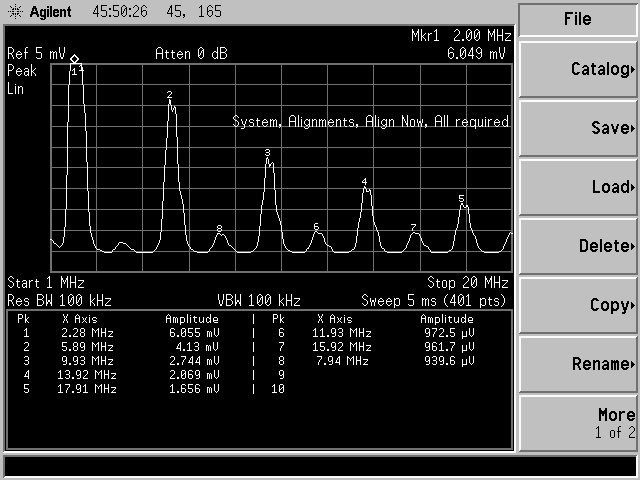
\includegraphics[width=0.7\textwidth]{daempfung_kurz.png}
  \caption{Die Fast-Fourier-Transformation eines Rechtecksignals,
    welches auf einem kurzen Kabel geführt wird, sodass die Dämpfung
    vernachlässigbar ist. Die Amplituden können direkt abgelesen
    werden.}
  \label{fig:daempfung_kurz}
\end{figure}
%
\begin{figure}[]
  \centering
  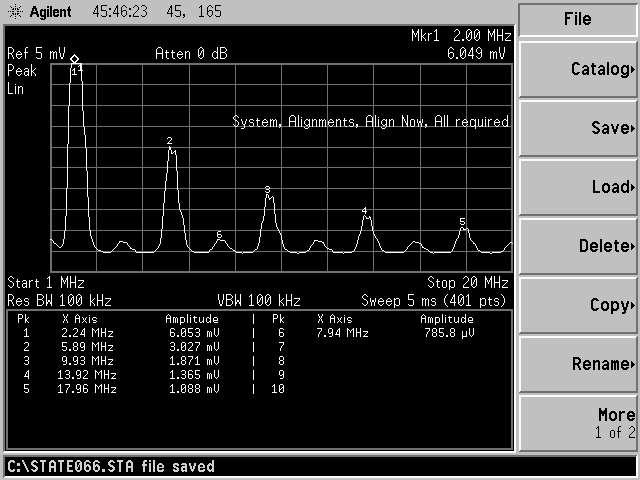
\includegraphics[width=0.7\textwidth]{daempfung_lang.png}
  \caption{Die Fast-Fourier-Transformation eines Rechtecksignals,
    welches auf einem langen Kabel geführt wird. Hierbei wird die in
    diesem Versuch verwendete Kabeltrommel genommen.  Es ist zu
    erkennen, dass die Amplituden, bis auf die erste, kleiner sind. Dies
    kommt durch die erhöhte Dämpfung dieses Kabels zustande.}
  \label{fig:daempfung_lang}
\end{figure}
%
\begin{table}[h]
  \centering
\setlength{\tabcolsep}{0.5cm}
  \begin{tabular}{cccc}
    \toprule
    ${U}_\text{ungedämpft}${/}\si{\milli\volt}&${U}_\text{gedämpft}{ /}\si{\milli\volt}$&
    {ln (}$\frac{{U}_\text{ungedämpft}}{{U}_\text{gedämpft}}${)}&
    $\alpha${/}\si{\per\metre}\\
    \midrule
    \SI{6.055(60)}{}&\SI{6.053(60)}{}&\SI{3e-4}{}$\pm$\SI{1e-2}{}
    &\SI{4.0e-6}{}$\pm$\SI{2e-4}{}\\
    \SI{4.130(41)}{}&\SI{3.027(30)}{}&\SI{0.31(1)}{}&\SI{0.0038(4)}{}\\
    \SI{2.744(27)}{}&\SI{1.871(18)}{}&\SI{0.38(1)}{}&\SI{0.0047(5)}{}\\
    \SI{2.069(20)}{}&\SI{1.365(13)}{}&\SI{0.42(1)}{}&\SI{0.005(5)}{}\\
    \SI{1.656(16)}{}&\SI{1.088(10)}{}&\SI{0.42(1)}{}&\SI{0.0051(5)}{}\\
    \midrule
    \multicolumn{2}{c}{Mittelwerte: }&\SI{0.31(7)}{}&\SI{0.004(1)}{}\\
    \bottomrule
  \end{tabular}
  \caption{Diese Tabelle führt die sich durch die 
    Fast-Fourier-Transformation ergebenden Amplituden auf.
    Damit wird die Dämpfung, sowie die Dämpfungskonstante als 
    Dämpfung pro Länge errechnet.}
  \label{tab:daempfung}
\end{table}
\FloatBarrier
%
\subsection{Mehrfacheflexion}
%
Nun wird das Signal untersucht, welches entsteht, wenn zwei Kabel mit
unterschiedlichen ohmschen Widerständen in Reihe geschaltet werden. Das
erste Kabel besitzt einen ohmschen Widerstand von \SI{50}{\ohm}, das
zweite \SI{75}{\ohm}.  Abbildung~\ref{fig:impulsfahrplan} zeigt den
dazugehörigen Impulsfahrplan, Abbildung~\ref{fig:mehrfachreflex} das mit
einem Oszilloskopen aufgenommene Bild.  Tabelle~\ref{tab:mehrfachreflex}
enthält die gemessenen Sprunghöhen in der Spannung und die daraus
berechneten Reflexionskoeffizienten.  Dabei bezeichnet $\Gamma_{50}$ den
Reflexionsfaktor am Anfang des \SI{50}{\ohm} Kabels und $\Gamma_{75}$
entsprechend den Reflexionsfaktor am Anfang des \SI{75}{\ohm} Kabels 
und $\Gamma_\text{E}$ den Reflexionsfaktor des offenen Endes.\\
Der erste Sprung in der Spannung bezeichnet die Eingangsspannung, 
was durch Gleichung~\eqref{eq:sprung1} ausgedrückt wird.
Nach längerer Rechnung und Beachtung der Phasensprünge des Signals 
ergeben sich für die Reflexionsfaktoren die in den 
Gleichungen~\eqref{eq:gamma75},~\eqref{eq:gammae} 
und~\eqref{eq:gamma50} angegebenen Formeln.\\
%
\begin{equation}
  \text{Sprung1} = U_0
  \label{eq:sprung1}
\end{equation}
%
\begin{equation}
  \Gamma_{75} = \frac{\text{Sprung2}}{\text{Sprung1}}
  \label{eq:gamma75}
\end{equation}
%
\begin{equation}
 \Gamma_\text{E} = \sqrt{\frac{\text{Sprung3}^2 -\text{Sprung2}\cdot \text{Sprung4}}
{\text{Sprung1}^2 -\text{Sprung2}^2}}
  \label{eq:gammae}
\end{equation}
%
\begin{equation}
\Gamma_{50} = \frac{\text{Sprung3}\cdot \text{Sprung1}}
{\text{Sprung2}^2}
-\Gamma_\text{E}\frac{\text{Sprung1}^2}{\text{Sprung2}^2}
+\Gamma_\text{E}
\label{eq:gamma50}
\end{equation}
%
\begin{figure}[]
  \centering
  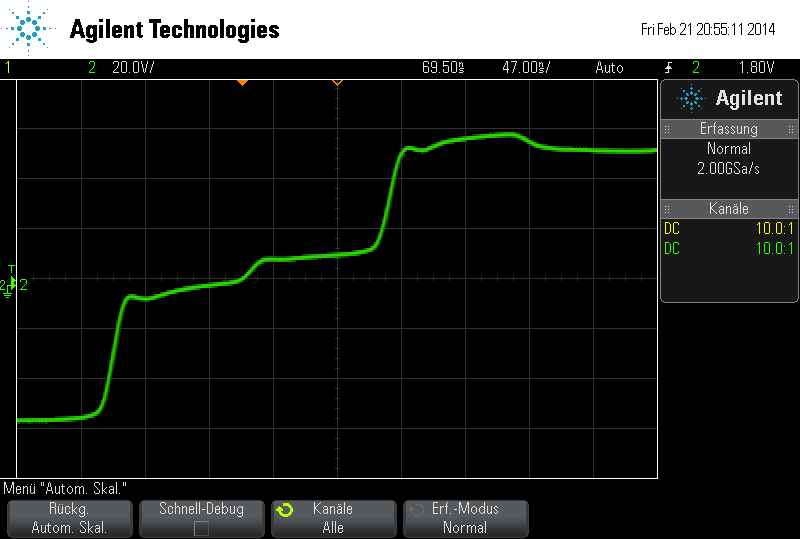
\includegraphics[width=0.8\textwidth]{reflex.png}
  \caption{Das Oszilloskopenbild bei Mehrfachreflexion. Es sind Vieri
    ausgeprägte Sprünge zu sehen. Die Schwankungen in der Spannung
    zwischen diesen Sprüngen ist auf das schlecht generierte
    Rechtecksignal des Funktionengenerators zurückzuführen.}
  \label{fig:mehrfachreflex}
\end{figure}
%
\begin{table}[h]
  \centering
  \begin{tabular}{SSSS}
    \toprule
    {Sprung Nr.}&{Sprunghöhe/}\si{\volt}&
    {Größe}&{Wert}\\
    \cmidrule(r){1-2} \cmidrule(l){3-4}
    1&50&{$U_0$}&50\si{\volt}\\
    2&8.2&{$\Gamma_{75}$}&0.16\\
    3&44.5&{$\Gamma_{E}$}&0.92\\
    4&-8.6&{$\Gamma_{50}$}&-0.13\\
    \bottomrule
  \end{tabular}
  \caption{Sprunghöhen und die daraus resultierenden 
    Reflexionsfaktoren bei Mehrfachreflexion.}
  \label{tab:mehrfachreflex}
\end{table}
%
\FloatBarrier
%
\subsection{Verschiedene Abschlusswiderstände}
%
In diesem Abschnitt werden die erhaltenen Signalspannungen für
verschiedene unbekannte Abschlusswiderstände mit den im Theorieteil
berechneten Signalspannungen verglichen, um so auf die Art des
Abschlusses und die dazugehörige Zeitkonstante zu schliessen.  Dazu
werden die im Theorieteil gefundenen Funktionen durch Messwerte
gefittet, die zuvor mithilfe der Cursorfunktion des im Versuch
verwendeten Oszilloskopen bestimmt wurden.\footnote{Zum Fitten der
  Messwerte wird die Funktion \texttt{scipy.optimize.curve\_fit} aus der
  Bibliothek \texttt{scipy-0.10.1} verwendet} Dabei ist zu beachten,
dass sich das reflektierte Signal mit dem einlaufenden Signal
überlagtert.  Tabelle~\ref{tab:fit_messwerte} beinhaltet die für die
verschiedenen Signalspannungen abgelesenen Messwerte.  Die Paragraphen
sind nach den verwendeten Kästen und Buchsen benannt.
%
\begin{table}[h!]
  \centering
  \begin{tabular}{SSSSSS}
    \toprule
    \multicolumn{2}{c}{Kasten 2 Buchse 3}&
    \multicolumn{2}{c}{Kasten 2 Buchse 4}&
    \multicolumn{2}{c}{Kasten 3 Buchse 6}\\
    \cmidrule(r){1-2} \cmidrule(rl){3-4} \cmidrule(l){5-6}
    {Zeit t /}\si{\nano\second}&{U /}\si{\volt}&
    {Zeit t /}\si{\nano\second}&{U /}\si{\volt}&
    {Zeit t /}\si{\nano\second}&{U /}\si{\volt}\\
    \midrule
    0&83.25&0&44.0&0&10.2\\
    10&69.0&130&41.7&280&18.2\\
    20&56.0&280&39.5&500&25.7\\
    30&48.0&470&36.2&760&34.7\\
    50&33.0&670&33.7&1180&47.2\\
    70&24.5&910&30.2&2260&69.0\\
    155&8.0&1360&24.2&3800&87.0\\
    300&5.8&2450&14.2&4740&93.5\\
    400&5.0&3540&8.7&6120&100.0\\
    &      &5000&3.2&9300&105.0\\
    &      &        &     &18660&107.0\\
    \bottomrule
  \end{tabular}
  \caption{Hier zu sehen sind die Messwerte, welche auf den Kurven 
    der sich ergebenden Signalspannungen liegen, wenn als Abschlüsse 
    des Kabels die über den Spalten genannten Kästen und Buchsen 
    verwendet werden.}
  \label{tab:fit_messwerte}
\end{table}
%
\paragraph{Kasten 2, Buchse 3}
Der sich bei diesem Abschluss ergebende Signalverlauf ist in
Bild~\ref{fig:k2b3} zu sehen. Der Fit mit der
Funktion~\eqref{eq:ind_ohm_reflex}, welche zu dem in Reihe geschalteten
ohmschen Widerstand und einer Induktivität gehört, liefert das beste
Ergebnis. Das Ergebnis dieses Fits ist in Formel~\eqref{eq:fit_k2b3}
wiedergegeben.  Daraus ergeben sich bei einem Wellenwiderstand des 
Kabels von $Z_0 =$ \SI{50}{\ohm} die Induktivität und der Widerstand 
des Abschlusses in~\eqref{eq:zeit_k2b3}. Die dazugehörige 
Zeitkonstante ist ebenfalls angegeben. 
Die Fehler für die Induktivität und den Widerstand durch die 
Fitfunktion sind gigantisch und übersteigen die sich durch den Fit 
ergebenden Fehler um mehrere Größenordnungen. 
Deswegen sind diese 
hier nicht angegeben. Für einen Grund dieser Fehler sei auf 
die Sektion Diskussion verwiesen. Bei allen folgenden Abschlüssen 
zeigt sich das selbe Verhalten.\\
Der Fehler für die Zeitkonstante wird durch einen seperaten Fit mit 
der Zeitkonstante als eigenen Anpassungsparameter ermittelt.\\
Der Plot in Abb.~\ref{fig:k2b3} zeigt die gefittete Kurve durch Punkte, die am
Oszilloskop aus dem Signalverlauf abgelesen wurden.
%
\begin{equation}
  U(t) = \SI{41.625}{\volt}\cdot\left(2 - 
    1.87\left(1-\exp{\left(\frac{-t}{\SI{48.9}{\nano\second}}\right)}
    \right)\right)
  \label{eq:fit_k2b3}
\end{equation}
%
\begin{equation}
  \tau = \frac{L}{Z_0 + R} = \frac{\SI{44.8}{\micro\henry}}
{\SI{50}{\ohm} + \SI{846}{\ohm}} 
=\SI{48.9(6)}{\nano\second}
  \label{eq:zeit_k2b3}
\end{equation}
%
\begin{figure}[]
  \centering
  \begin{subfigure}{0.45\textwidth}
    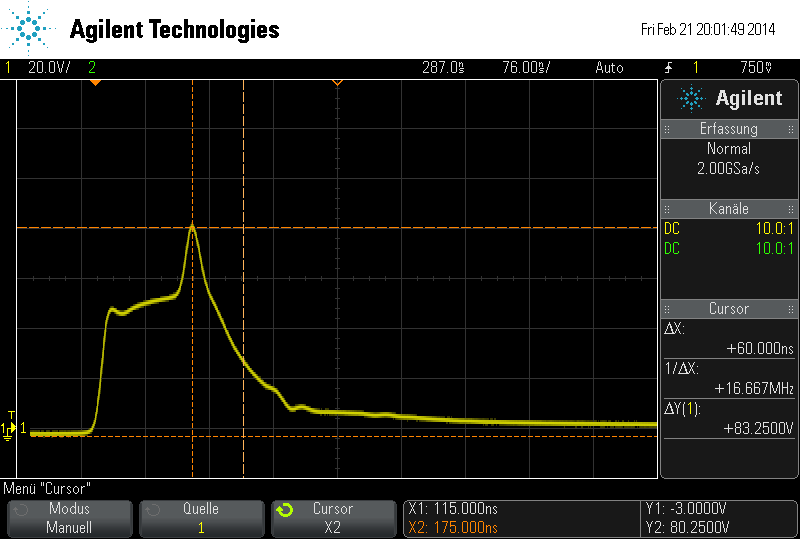
\includegraphics[width=\textwidth]{k2b3.png}
  \end{subfigure}
  \quad
  \begin{subfigure}{0.45\textwidth}
    \includegraphics[width=\textwidth]{fit_k2b3.pdf}
  \end{subfigure}

  \caption{Hier ist das vom Oszilloskop gemessene Signal der Buchse 3
    von Kasten 2 und der Plot, der die aus dem Abbild des Oszilloskops
    entnommenen Daten mit ihrer Regressionskurve zeigt, abgebildet.  Es
    wird eine Reihenschaltung aus ohmschen Widerstand und Induktivität
    angenommen.}
  \label{fig:k2b3}
\end{figure}

\paragraph{Kasten 2, Buchse 4}
Bild~\ref{fig:k2b4} zeigt den sich ergebenden Signalverlauf bei diesem
Abschluss.  Wie bei dem vorherigen Abschluss passt der Fit mit der
Funktion~\eqref{eq:ind_ohm_reflex}, also dem in Reihe geschalteten
ohmschen Widerstand und einer Induktivität, am besten.  Der Fit ergibt
Formel~\eqref{eq:fit_k2b4}.  Hier ergeben sich die Induktivität, der 
Widerstand und die Zeitkonstante in~\eqref{eq:zeit_k2b4}.
Der Fehler der Zeitkonstanten wird wieder mit einem seperaten 
Fit mit der Zeitkonstanten als Parameter bestimmt. 
Messwerte und Fit sind in
Abb.~\ref{fig:k2b4} zu sehen.
%
\begin{equation}
  U(t) = \SI{22.0}{\volt}\cdot\left(2 - 
    2.182\left(1-\exp{\left(\frac{-t}{\SI{2.62}{\micro\second}}\right)}
    \right)\right)
  \label{eq:fit_k2b4}
\end{equation}
%
\begin{equation}
  \tau = \frac{L}{Z_0 + R} = 
\frac{\SI{21.8}{\milli\henry}}{\SI{50}{\ohm} + 
\SI{8260}{\ohm}} =\SI{2.62(8)}{\micro\second}
  \label{eq:zeit_k2b4}
\end{equation}
%
\begin{figure}[]
  \centering

  \begin{subfigure}{0.45\textwidth}
    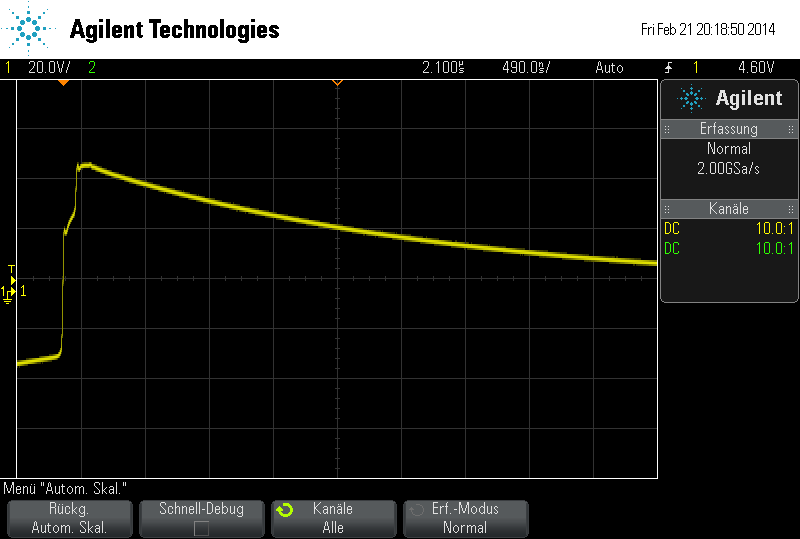
\includegraphics[width=\textwidth]{k2b4.png}
  \end{subfigure}
  \quad
  \begin{subfigure}{0.45\textwidth}
    \includegraphics[width=\textwidth]{fit_k2b4.pdf}
  \end{subfigure}

  \caption{Fit durch am Oszilloskop abgelesenen Punkten bei
    Kabelabschluss Kasten Zwei, Buchse Vier.  Aufgenommener
    Signalverlauf bei Kabelabschluss an Kasten Zwei, Buchse Vier. Auch
    bei diesem Abschluss wird eine Reihenschaltung von ohmschen
    Widerstand und Induktivität festgestellt.}
  \label{fig:k2b4}
\end{figure}

\paragraph{Kasten 3, Buchse 6}
Das Signal des letzten Abschlusses ist in Bild~\ref{fig:k3b6} zu sehen.
Diesmal passt der Fit mit der Funktion~\eqref{eq:cap_ohm_reflex}, dem in
Reihe geschalteten ohmschen Widerstand und einer Kapazität, sehr gut.
Formel~\eqref{eq:fit_k3b6} gibt das Ergebnis des Fits an.  Bei diesem
Abschluss ergeben sich Widerstand und Kapazität, sowie die 
Zeitkonstante in~\eqref{eq:zeit_k3b6}. Der  Plot
in Abb.~\ref{fig:k3b6} zeigt Messwerte und gefittete Kurve.
%
\begin{equation}
  U(t) = \SI{53.9}{\volt}\cdot\left(2 + 
    \left(-8.1 - 1\right)\exp{\left(\frac{-t}
{\SI{2.51}{\micro\second}}\right)}\right)
  \label{eq:fit_k3b6}
\end{equation}
%
\begin{equation}
  \tau = (Z_0 + R)C = 
(\SI{50}{\ohm}+\SI{436}{\ohm})\cdot\SI{5.2}{\nano\farad}= 
\SI{2.51(6)}{\micro\second}
  \label{eq:zeit_k3b6}
\end{equation}
%
\begin{figure}[]
  \centering

  \begin{subfigure}{0.45\textwidth}
    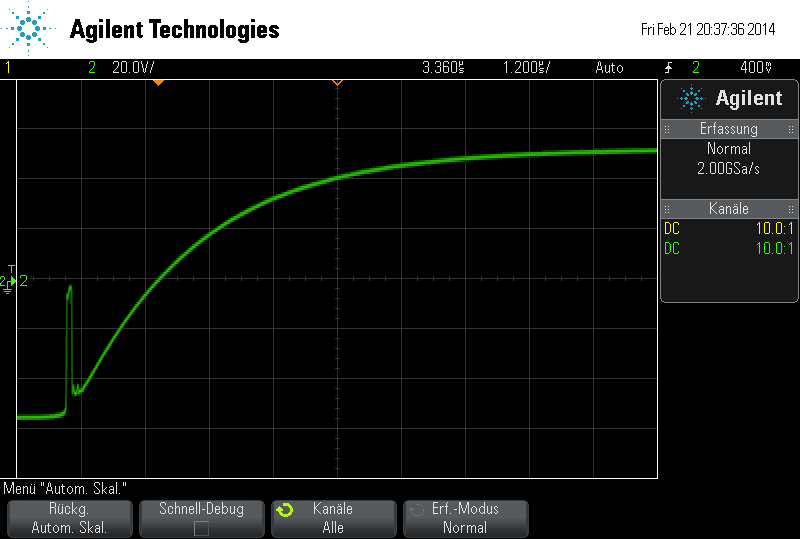
\includegraphics[width=\textwidth]{k3b6.png}
  \end{subfigure}
  \quad
  \begin{subfigure}{0.45\textwidth}
    \includegraphics[width=\textwidth]{fit_k3b6.pdf}
  \end{subfigure}

  \caption{Messwerte und durch diese für den Abschluss mit Kasten Drei,
    Buchse Sechs.  Dieser Signalverlauf ergibt sich, wenn als
    Kabelabschluss Kasten Drei, Buchse Sechs gewählt wird. Diesmal
    handelt es sich um eine Reihenschaltung aus ohmschen Widerstand und
    Kapazität.}
  \label{fig:k3b6}
\end{figure}
%